\documentclass[a4paper,12pt]{article}

\usepackage[utf8]{inputenc} 
\usepackage{amsmath}
\usepackage[a4paper, margin=0.9in]{geometry} % Adjust the margin here
\usepackage{multirow}
\usepackage{nopageno}
\usepackage{graphicx} % Add this line to include graphics
\setlength{\parindent}{0pt} % Set global no indent
    
\title{{\large Department of Physics, FNSPE, CTU in Prague} \\
                  02YMECH - Mechanics \\ 
          {\Large \textbf{Midterm 1}}\vspace{-1cm}}
\date{7.11.2025 / 14:00 - 16:00}
\author{}

\begin{document}

\maketitle


\vspace*{0.5cm}
\noindent
\textbf{Q1:} Three point particles collide instantaneously at the origin with no external force. Their masses and pre-collision velocities are
\[
m_1 = 1\,\mathrm{kg}, \qquad 
m_2 = 2\,\mathrm{kg}, \qquad
m_3 = 3\,\mathrm{kg},
\]
\[
\vec{v}_{1i} = (2,0,1)\,\mathrm{m/s}, \qquad
\vec{v}_{2i} = (-1,1,0)\,\mathrm{m/s}, \qquad
\vec{v}_{3i} = (0,-2,3)\,\mathrm{m/s}.
\]
Immediately \emph{after} the collision, particle~1 moves along $\hat{\imath}$, particle~2 along 
\(-\hat{\jmath}\), and particle~3 along \(+\hat{k}\).  
\begin{enumerate}
\item[(a)] Determine the velocities after the collision: 
\(\vec{v}_{1f}, \vec{v}_{2f}, \vec{v}_{3f}\). --- \textit{0.6 points}
\item[(b)] Determine whether the collision is elastic or not. --- \textit{0.4 points}
\end{enumerate}

\vspace*{0.5cm}
\textbf{Q2:} A projectile with a mass $m$ strikes a wall with a velocity $v_1$ and exits from the other side with a velocity $v_2$ after penetrating the wall of thickness $d$. What was the average force $F$ acting on the projectile inside the wall? --- \textit{1 point}

\vspace*{0.5cm}
\begin{minipage}[t]{0.7\textwidth}
\textbf{Q3:} A mathematical pendulum with a length of $l$ is attached to the arm of a rotating carousel at a distance $d$ from its axis. The pendulum is deflected from its vertical position by an angle $\alpha$. Calculate the period of rotation for the carousel. --- \textit{1 point}
\end{minipage}%
\hfill
\begin{minipage}[t]{0.25\textwidth}
\vspace{-35pt}
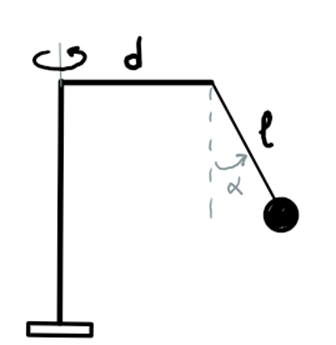
\includegraphics[width=\textwidth]{carousel.png}
\end{minipage}

\vspace*{0.5cm}
\textbf{Q4:} A particle of mass $m$ can move without friction along the  $x$-axis. At time $t = 0$, it is at rest at position $x = 0$. A force $F_x(t) = k\cos(\omega t)$ acts on it, where $k$ and $\omega$ are constants. 
\begin{itemize}
    \item[(a)] Determine the acceleration $a(t)$, the velocity $v(t)$, the displacement $x(t)$. --- \textit{0.6 points}
    \item[(b)] Determine the power delivered by the force at an arbitrary time $t$. --- \textit{0.4 points}
\end{itemize}


\end{document}

